\documentclass{article}

\usepackage{fancyhdr} % Required for custom headers
\usepackage{lastpage} % Required to determine the last page for the footer
\usepackage{extramarks} % Required for headers and footers
\usepackage[usenames,dvipsnames]{color} % Required for custom colors
\usepackage{graphicx} % Required to insert images
\usepackage{listings} % Required for insertion of code
\usepackage{courier} % Required for the courier font
\usepackage{lipsum} % Used for inserting dummy 'Lorem ipsum' text into the template
\usepackage{titling}
%\usepackage{hyperref}
\topmargin=-0.0in
\evensidemargin=0in
\oddsidemargin=0in
\textwidth=6.5in
\textheight=9.0in
\headsep=0.25in

\newcommand{\hmwkTitle}{Shape Categorization\\Final Report} % Assignment title
\newcommand{\hmwkClass}{Computer Vision} % Course/class Class/lecture time
\newcommand{\hmwkClassInstructor}{Prof. Dr.-Ing. Rainer Herpers} % Teacher/lecturer
\newcommand{\hmwkimage}{\centering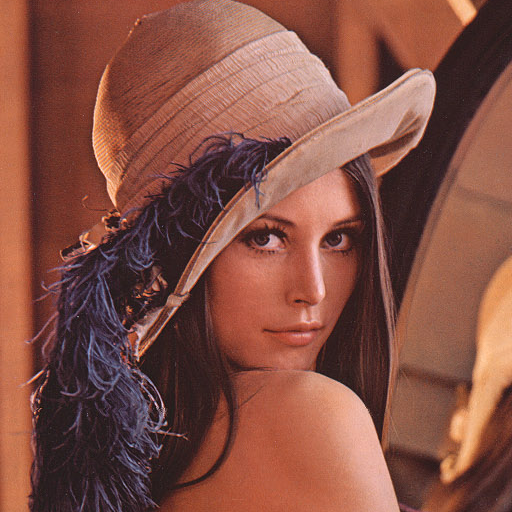
\includegraphics[draft=false, scale = 0.5]{images/lenna.png}}
\newcommand{\hmwkAuthorName}{Senthilkumar Sockalingam Kathiresan} % Your name
\newcommand{\hmwksecondauthor}{Yannick Weitz}
\newcommand{\hmwkfirstmat}{Matrikel Nr. 9030382}
\newcommand{\hmwksecondmat}{Matrikel Nr. 9030385}

%----------------------------------------------------------------------------------------
%	TITLE PAGE
%----------------------------------------------------------------------------------------


\title{
\vspace{2in}
\textmd{\textbf{\hmwkClass:\ \\ \hmwkTitle}}\\
\vspace{0.1in}\large{\hmwkClassInstructor\ }
\vspace{3in}
}

\author{\textbf{\hmwkAuthorName}, \hmwkfirstmat\\ \textbf{\hmwksecondauthor}, \hmwksecondmat}
\date{} % Insert date here if you want it to appear below your name

\begin{document}
\begin{titlepage}
\hmwkimage\\
\vspace{1in}
\textmd{\Huge\textbf{\hmwkClass:\ \\ \hmwkTitle}}\\
\vspace{0.1in}\large{\hmwkClassInstructor\ }
\vspace{3in}\\
\theauthor\
\thispagestyle{empty}
\end{titlepage}


\setcounter{page}{1}

\tableofcontents

\newpage

\section{Introduction}

\begin{itemize}
\item Objective / abstract goal, problem analysis
\end{itemize}

The Task that should be solved by this Computer Vision project is based on a Task taken from the Robocup@Work rulebook. The youBot should be able to fit a 3 dimensional piece into the correct 2 dimensional cavity.\\
In order to fit the part into the cavity, the correct cavity has to be determined first. The whole task is testing the perception as well as the manipulation ability of the youbot.\\
As given by the rule book of the Robocup@work:

\begin{quote}

single robot is used.  The robot is placed by the team freely within the arena.  The
objective of the task is to pick the objects which are placed on one service area and make a
precise-placement in the corresponding cavity at the service area with the special PPT platform
(an example configuration is illustrated in Figure
3.2).
The task consists of multiple grasp and place operations, possibly with base movement in be-
tween, which will, however, be short.  The task is finished once the objects are picked up and
placed in the corresponding cavities or when the time foreseen for the run ends.  Note that the
placement of the object in the cavity is finished when the object is fallen into the cavity (i.e.  at
least some part of the object has to touch ground floor underneath the cavity).
All objects to be transported in a run of a team and the corresponding cavities share the same
orientation, either horizontal or vertical.  This may vary between different teams and different
runs.[1]\\

\end{quote}

\section{Material and methods}

\begin{itemize}
\item Description of your setup and your data
\item Assumptions and prerequisites
\item Approach you are going to apply incl. motivation
\item Plan of attack, structure /decomposition of sub steps
\end{itemize}

\textbf{Prerequisites}\\

For this task the youBot will get the command to pick up a particular part from a toolbox, from the referee unit, and then drive back to the table, where the cavities are stored. This is where the project begins. The camera of the youBot is pointing at the table. Five out of twelve plates will be placed in a cavities inside the table, arranged in a row (fig. \ref{fig:row}). The background of the cavities inside the tiles will thus be black and the full tile will always be visible. The tiles themselves have a nearly white color and will be produced by a 3D printer. The size is fixed to $14cm^2$, with a thickness of  $1cm$ .\\
The object, that the youBot is holding is already recognized and known to the bot. There are 5 different objects available.\\
The cavities are always centered in the middle of the tile and will only correspond to only one particular orientation of the object.\\
The youBot is using a asus xtion pro live for this task. The camera will be positioned in front of the tiles, with different possible angles, always capturing all five tiles. \\
There will be no additional light source attached to the youBot, so shadows are possible.\\

\begin{figure}[h!]
\centering
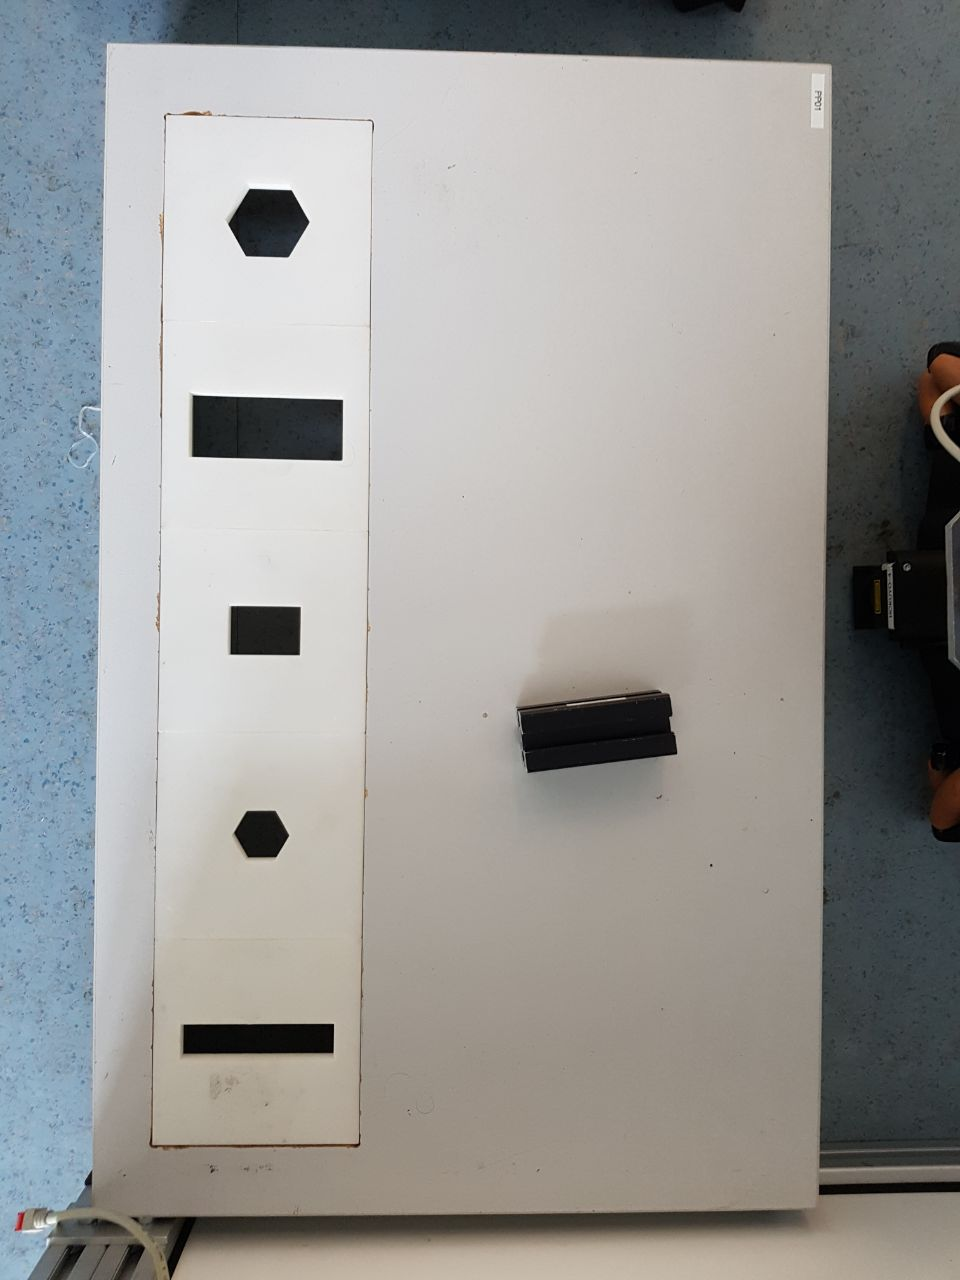
\includegraphics[scale=0.15,angle=270]{images/5tiles.jpeg}
\caption{Example of a set of five tiles arranged like they will be in the Robocup@Work competition.}
\label{fig:row}
\end{figure}

\textbf{General Approach}

As a preprocessing step the image input has to be normalized. Since it can't be assumed that the youBot will always provide a 90$^\circ$ top-down view of the tiles, the input image should should be transformed using homography. The new image after this step should only show an approximate of what the row of tiles would look like from the 90$^\circ$ top-down view. The result will then be further decomposed into the single tiles.\\
To classify the extracted tiles, a comparison between the tiles and a database is performed. The database consists of example images showing all the tiles in all possible configurations.\\

\textbf{Data}\\

Eight different datasets have been created for training purpose. All datasets show the same dataset specific setup from different angles. Five of the datasets consist of a collection of five tiles, placed into the table, with regular lighting, no occlusion and no other objects. The three remaining datasets have been created to test extreme conditions.\\
For the five regular sets, some tiles have specifically been chosen, while the rest is selected arbitrarily. The first set consists of simple shapes, where the focus is placed on differentiating between the same shape with a different size, which could give problems due to the similarity of the two shapes (fig. \ref{fig:datasets}, top, most left).\\
The second dataset is introducing more complex shapes, that could be harder to classify and recreate while using homography (fig. \ref{fig:datasets}, top, second from the left).\\
In the third datasets only small similar looking shapes have been chosen to test the algorithm for a number of similar shapes (fig. \ref{fig:datasets}, top, second from the right).\\
The fourth set shows four variations of the same 2 dimensional shape, that fit to different 3 dimensional objects (fig. \ref{fig:datasets}, top, most right).\\
The fifth set is used to determine how the algorithm works for similar shapes with different orientations (fig. \ref{fig:datasets}, bottom, most left).\\
For the three remaining sets the focus is set to special conditions rather then testing the algorithm for the distinction between different shapes.\\
In the sixth dataset, the number of tiles has been reduced to four in order to test border cases (fig. \ref{fig:datasets}, bottom, second from the left), the algorithm is not expected to solve this problem, it is just an additional case.\\
The Seventh set shows images that correspond to a problem that occurs if other areas in the image have the same color and shape of the cavities (fig. \ref{fig:datasets}, bottom, second form the right).\\
In the last dataset, the light-source has been switched of to create a darker image (fig. \ref{fig:datasets}, bottom, most right).\\
It can easily be seen, that each example image from the eight datasets has different areas of lighting, thus no dataset testing for shadows was necessary.
\begin{figure}[h!]
\begin{minipage}{\textwidth}
\centering
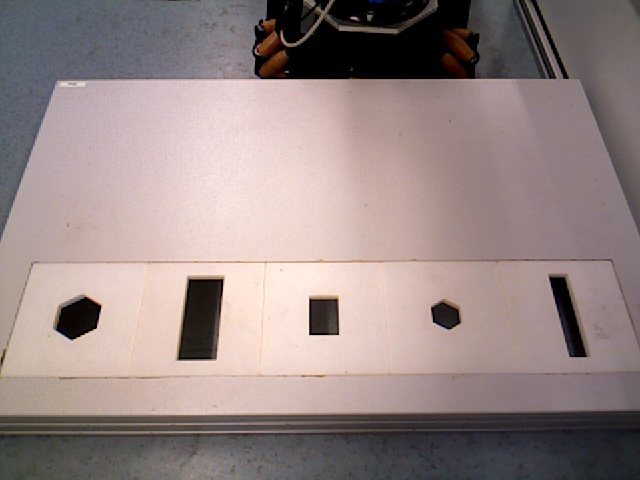
\includegraphics[scale=0.15]{images/First_set.jpg}\hspace{0.1cm}
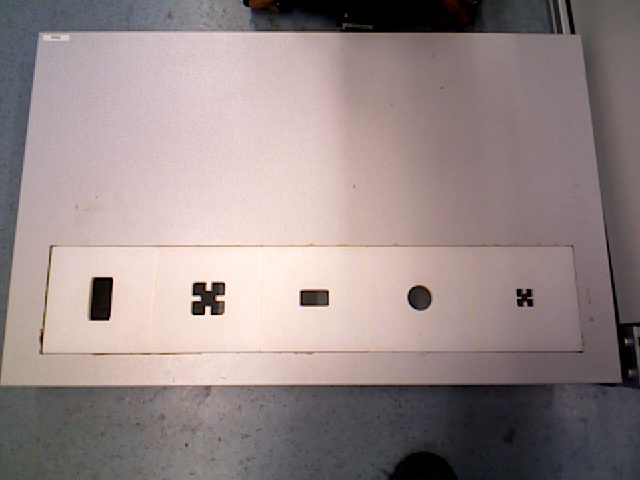
\includegraphics[scale=0.15]{images/Second_set.jpg}
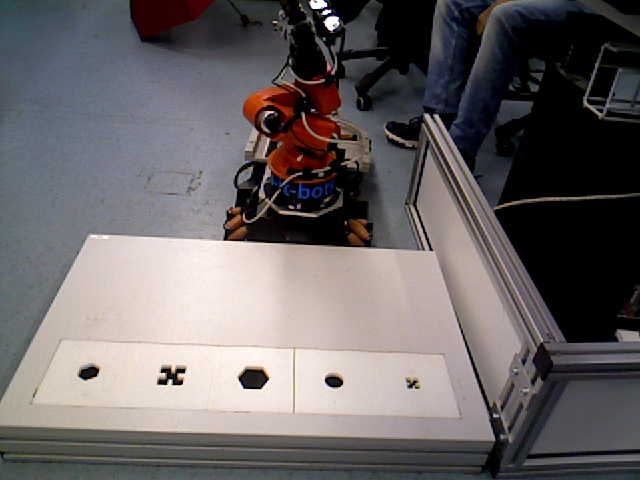
\includegraphics[scale=0.15]{images/Third_set.jpg}
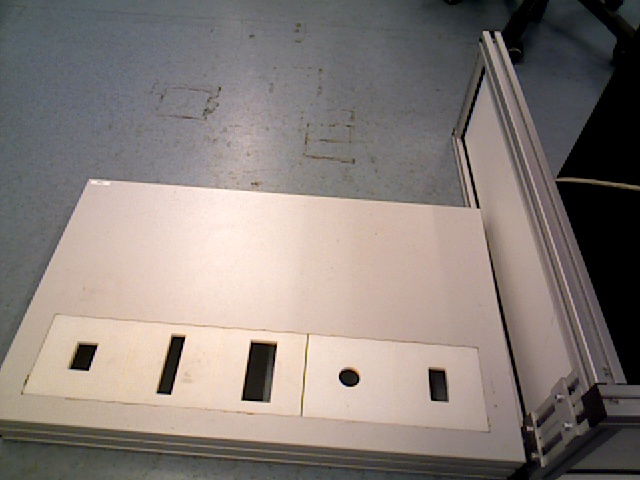
\includegraphics[scale=0.15]{images/Fourth_set.jpg}\vspace{0.1cm}
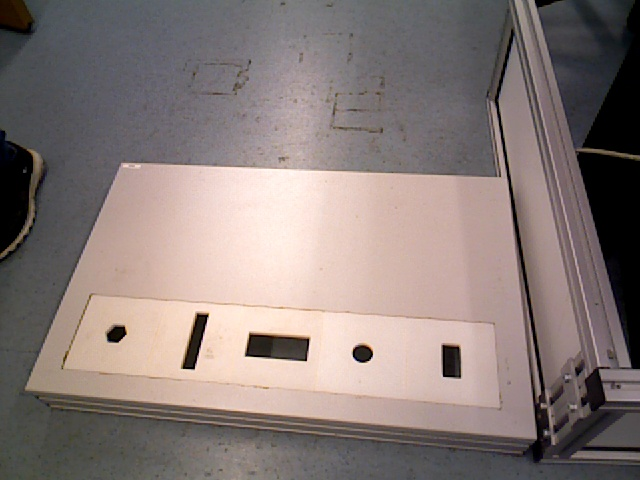
\includegraphics[scale=0.15]{images/Fifth_set.jpg}\hspace{0.1cm}
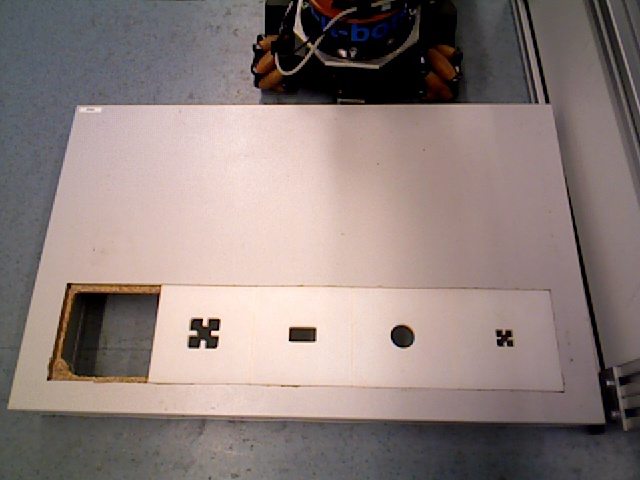
\includegraphics[scale=0.15]{images/Sixth_set.jpg}
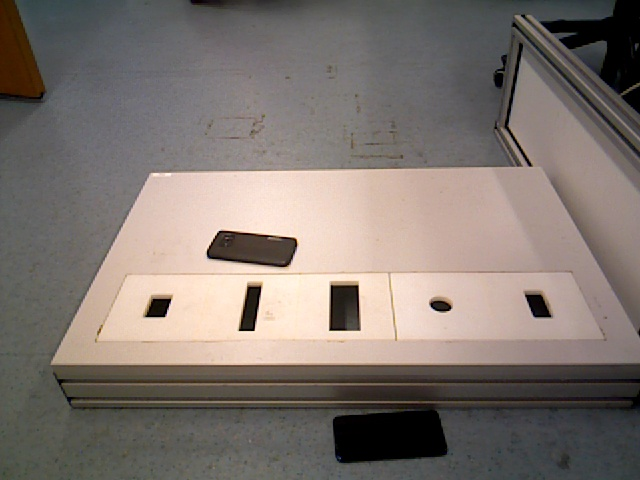
\includegraphics[scale=0.15]{images/Seventh_set.jpg}
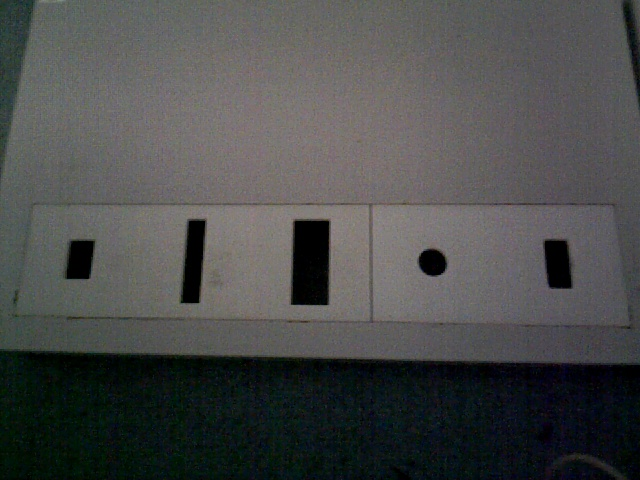
\includegraphics[scale=0.15]{images/Eigth_set.jpg}
\caption{Example images for the eight datasets, starting with one in the top left corner, to eight in the lower right.}
\label{fig:datasets}
\end{minipage}
\end{figure}

\section{Approach}

In order to normalize the input image and rectify the row of tiles, the first step is to crop the image and get rid of unnecessary information (fig. \ref{fig:original}). \\
\begin{figure}[h!]
\centering
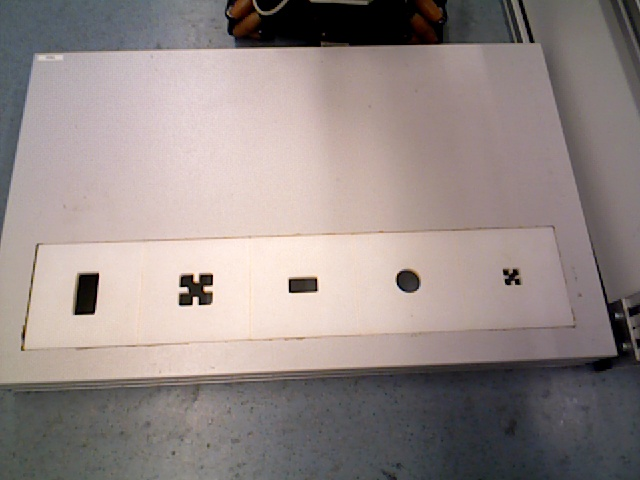
\includegraphics[scale=0.3]{images/frame01.jpg}
\caption{The Original image containing irrelevant information, like the table or small parts of the robot.}
\label{fig:original}
\end{figure}

so at first the area that should be cropped has to be determined. Since the images are in general a lot brighter than the cavities, an edge filter is applied (fig. \ref{fig:edges}). Threshold and adaptive threshold have been tested but didn't deliver a good result.\\
\begin{figure}[h!]
\centering
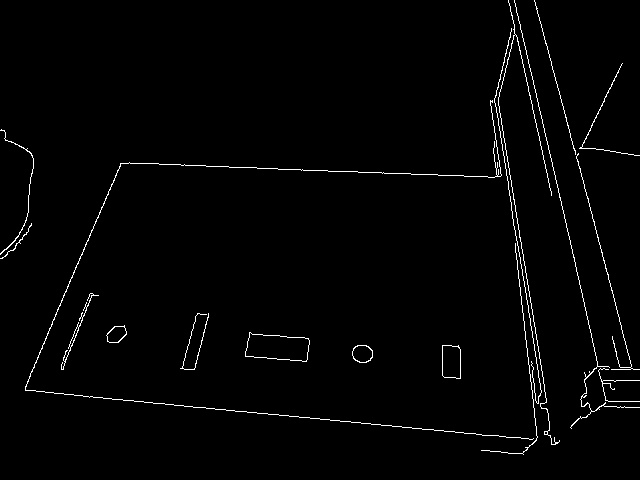
\includegraphics[scale=0.3]{images/edges.jpg}
\caption{The image after a canny edge filter has been applied.}
\label{fig:edges}
\end{figure}
All the contours of the processed image are extracted and the pixel coordinates of the center points are stored (fig. \ref{fig:cavities}). Since all contours should lie in the middle of the tiles, the centers of the cavities should lie in a line consisting of five equally spaces points. \\
\begin{figure}[h!]
\centering
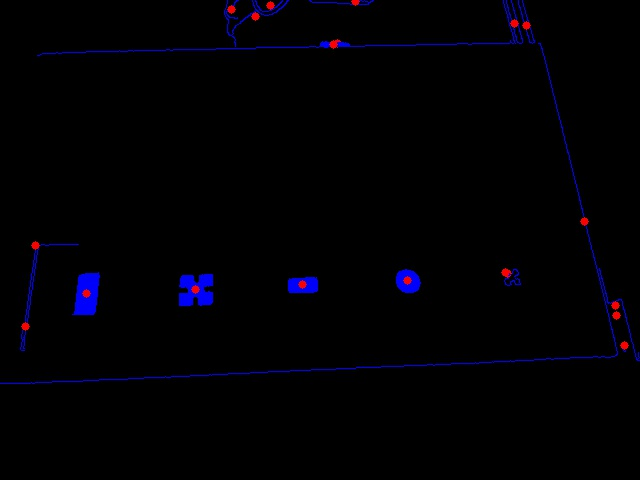
\includegraphics[scale=0.3]{images/cavitycontours.jpg}
\caption{All the extracted contours from the edge detection image.}
\label{fig:cavities}
\end{figure}
To find the five points that correspond to these centers, a line is drawn between all extracted centers from substep one. From all the lines where at least five points lie closely on the same line, the one is chosen where the error between the points and the line is the least (fig. \ref{fig:line}). This has proven to give the correct line for all tested images. Since we search for the minimum distance, lines with five points are preferred over lines with more points, so by default lines with to many points get ruled out.\\
\begin{figure}[h!]
\centering
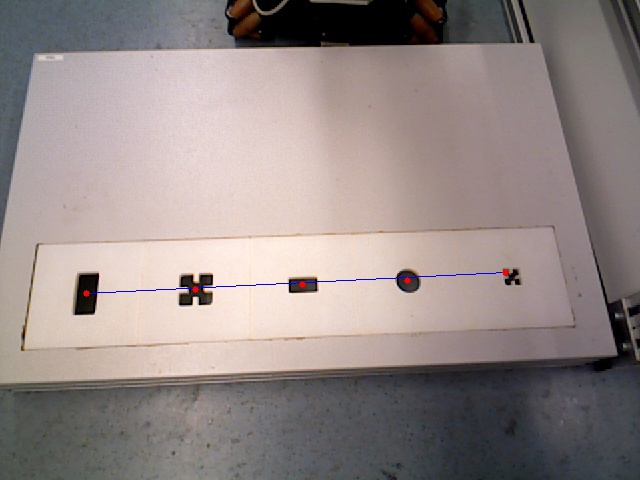
\includegraphics[scale=0.3]{images/line.jpg}
\caption{The five points that lie closest to a line have been extracted.}
\label{fig:line}
\end{figure}
We know that all tiles have the same dimensions. Thus, the next step aims to find a correspondence between the pixels and the distance, or pixels per centimeter. The center points of the cavities are expected to lie in the center of the tile. It follows, that the distance between two neighboring centers is equal to $14cm$.Hence, The approximate pixel equivalent to $14cm$ is calculated by getting the mean distance between two neighboring tile centers.\\
Now the image can be cropped by using (fig. \ref{fig:cropped}):
\begin{equation}
cropped \, image = image[min(x)-\frac{\mu_{dist}}{2}:max(x)+\frac{\mu_{dist}}{2},min(y)-\frac{\mu_{dist}}{2}:max(y)+\frac{\mu_{dist}}{2}]
\end{equation}
Where:
\begin{quote}
$\frac{\mu_{dist}}{2}$ = Pixel per 7 Centimeter, plus some additional term to compensate the angular orientation of the five tiles\\
$min(x)$ = Minimum x value of all center points\\
$max(x)$ = Maximum x value of all center points\\
$min(y)$ = Minimum y value of all center points\\
$max(y)$ = Maximum y value of all center points\\
\end{quote}
\begin{figure}[h!]
\centering
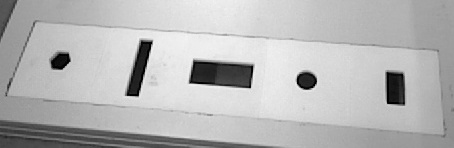
\includegraphics[scale=0.3]{images/cropped.jpg}
\caption{A lot of irrelevant information has been cropped out of the image.}
\label{fig:cropped}
\end{figure}
To extract now the corners of the five tile row, the adaptive threshold filter is applied to the cropped image, since this has proven to give a good differentiation between the five tile row and the background. Again the contours of the image are extracted, this time with a limitation of the area, that the contour should enclose (fig. \ref{fig:five}). \\
\begin{figure}[h!]
\centering
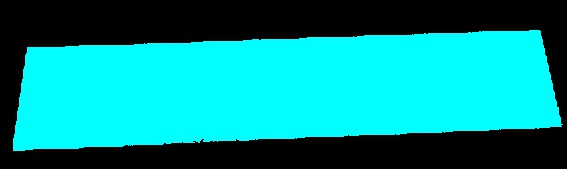
\includegraphics[scale=0.3]{images/5tiles.jpg}
\caption{The contour of the image that corresponds to the biggest area of the cropped image.}
\label{fig:five}
\end{figure}
The low resolution of the image makes it hard to extract the four corners immediately. To get only the four corner points of the tile row, a number of possible corner points is extracted from the contour. These points are then ... (fig. \ref{fig:points})\\
\begin{figure}[h!]
\centering
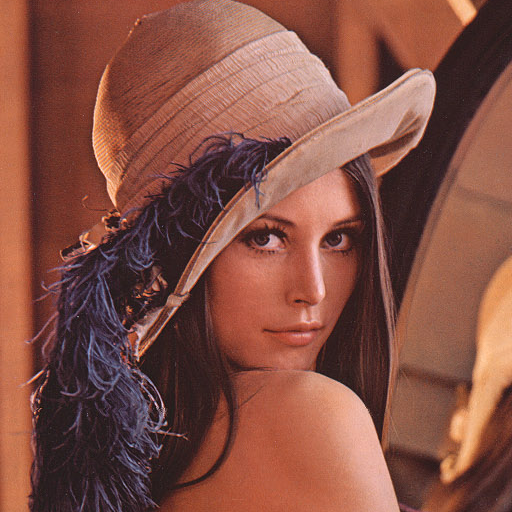
\includegraphics[scale=0.3]{images/lenna.png}
\caption{Only four corner points remain, enclosing the whole contour of the five tiles.}
\label{fig:points}
\end{figure}
The four points are used to transform the perspective of the tiles to create and artificial top-down image containing only the five tiles (fig. \ref{fig:homograph}).\\
\begin{figure}[h!]
\centering
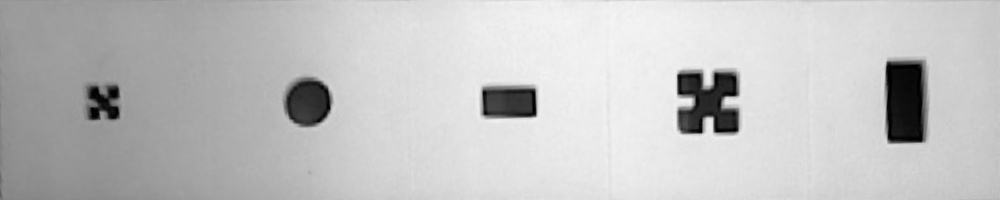
\includegraphics[scale=0.3]{images/homography.jpg}
\caption{An artifical top-down view of the five tiles.}
\label{fig:homograph}
\end{figure}
The resulting image is then divided into five equal parts and the images are stored (fig. \ref{fig:individ}).\\
\begin{figure}[h!]
\begin{minipage}{\textwidth}
\centering
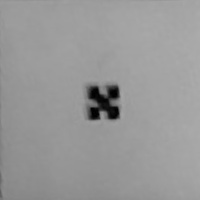
\includegraphics[scale=0.3]{images/tile0.jpg}
\hspace{0.1cm}
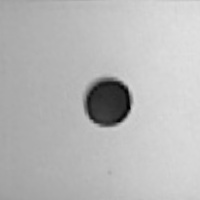
\includegraphics[scale=0.3]{images/tile1.jpg}
\hspace{0.1cm}
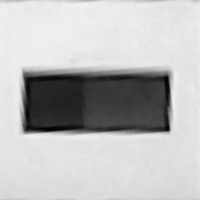
\includegraphics[scale=0.3]{images/tile2.jpg}
\hspace{0.1cm}
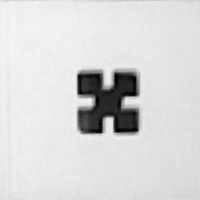
\includegraphics[scale=0.3]{images/tile3.jpg}
\hspace{0.1cm}
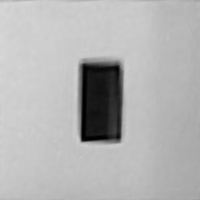
\includegraphics[scale=0.3]{images/tile4.jpg}
\caption{The five cropped individual images of the tiles.}
\label{fig:individ}
\end{minipage}
\end{figure}


\section{Evaluation and results}

\begin{itemize}
\item Test /Evaluation design
\item Riscs
\end{itemize}

\begin{thebibliography}{99}
	\bibitem{first} Robocup @work rulebook, p. 35. Robocup-rulebook2017
	\bibitem{second} ? 
	\end{thebibliography}
\end{document}